\setlength{\columnsep}{3pt}
\begin{flushleft}
	\bigskip
	\begin{itemize}
		\item Sticky bit can be applied only on directories.
		\item Content of directory having sticky bit on it \textbf{can be only deleted by root or the user who created that file.}
		\item Sticky bit is applicable only on \textbf{other users.} 
		\item Sticky bit is denoted as \textbf{'t'} for other, if \textbf{other} has execute permission.
		\begin{figure}[h!]
			\centering
			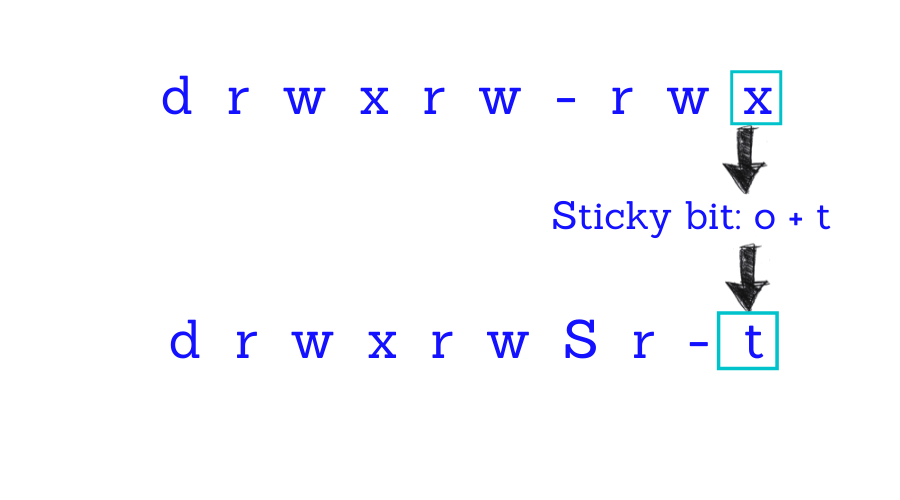
\includegraphics[scale=0.4]{content/chapter6/images/22.png}
			\caption{Sticky bit with execute permission}
			\label{fig:acl_example_9}
		\end{figure}
		\item Sticky bit is denoted as \textbf{'T'} for other, if \textbf{other} has no execute permission.
		\begin{figure}[h!]
			\centering
			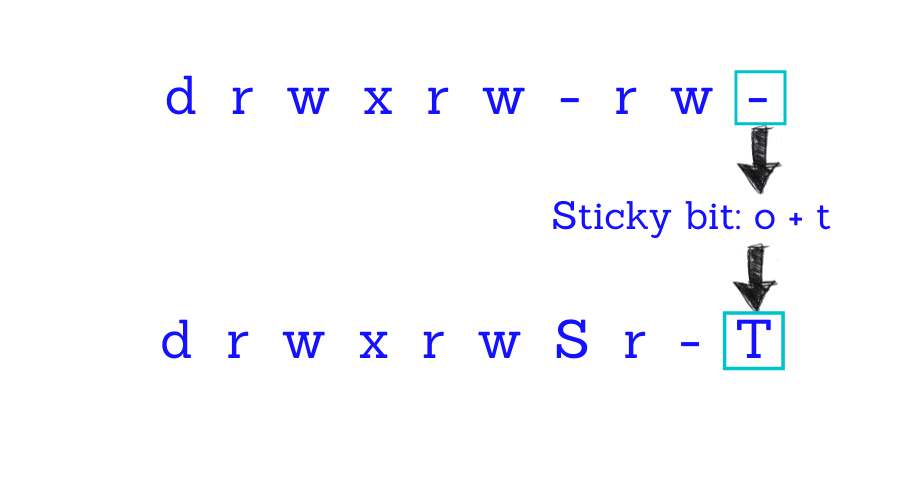
\includegraphics[scale=0.4]{content/chapter6/images/23.png}
			\caption{Sticky bit without execute permission}
			\label{fig:acl_example_8}
		\end{figure}
		
		\item Eg: \textbf{/tmp} directory is having sticky bit permission on it, so that only root or the owner of the files under /tmp can delete it's content.
		/tmp/.
		\item Octal representation of sticky bit is \textbf{1}.	
	\end{itemize}
\newpage

\paragraph{How to apply sticky bit permission?}
\bigskip
\begin{tcolorbox}[breakable,notitle,boxrule=0pt,colback=pink,colframe=pink]
	\color{black}
	\fontdimen2\font=1em
	Syntax: chmod o+t directory\_name
	\fontdimen2\font=4pt
\end{tcolorbox}
Eg: Create a folder named \textbf{/opt/dump} and provide it with permission \textbf{757} and \textbf{sticky bit}.
\begin{tcolorbox}[breakable,notitle,boxrule=-0pt,colback=black,colframe=black]
	\color{green}
	\fontdimen2\font=1em
	\# mkdir /opt/dump/
	\newline
	\$ chmod o+t,u=rwx,g=r-x,o+rwx /opt/dump/
	\newline
	or
	\newline
	\$ chmod 1757 /opt/dump/
	\fontdimen2\font=4pt
\end{tcolorbox}
As local user named "raj", \textbf{create a file named /opt/dump/sample.txt}.
\begin{tcolorbox}[breakable,notitle,boxrule=-0pt,colback=black,colframe=black]
	\color{green}
	\fontdimen2\font=1em
	\# su - raj
	\newline
	\$ touch /opt/dump/sample.txt
	\fontdimen2\font=4pt
\end{tcolorbox}

As local user "ravi", delete the file \textbf{/opt/dump/sample.txt} and confirm below error:
\begin{tcolorbox}[breakable,notitle,boxrule=-0pt,colback=black,colframe=black]
	\color{green}
	\fontdimen2\font=1em
	\# su - ravi
	\newline
	\$ rm /opt/dump/sample.txt
	\color{white}
	\newline
	rm: cannot remove '/opt/test/sample.txt': Operation not permitted
	\fontdimen2\font=4pt
\end{tcolorbox}

\newpage
\paragraph{How to remove sticky bit permission?}
\bigskip
\begin{tcolorbox}[breakable,notitle,boxrule=0pt,colback=pink,colframe=pink]
	\color{black}
	\fontdimen2\font=1em
	Syntax: chmod o-t directory\_name
	\fontdimen2\font=4pt
\end{tcolorbox}
Eg:
\begin{tcolorbox}[breakable,notitle,boxrule=-0pt,colback=black,colframe=black]
	\color{green}
	\fontdimen2\font=1em
	\$ chmod o-t /opt/dump/
	\newline
	or
	\newline
	\$ chmod 0757 /opt/dump/
	\fontdimen2\font=4pt
\end{tcolorbox}
	
	
\end{flushleft}

\newpage

